\documentclass[11pt]{article}
\usepackage[a4paper,left=2.5cm,right=2cm,top=2.5cm,bottom=2.5cm]{geometry}
\usepackage[T1]{fontenc}
\usepackage{xcolor}
\usepackage{amssymb}
\usepackage{listings}
\usepackage{graphicx}
\usepackage{amsmath, mathpazo}

\usepackage[pdfauthor={Christoph Sonntag},
            pdftitle={Christoph Sonntag's Assignment 1},
            pdfkeywords={}]{hyperref}
\usepackage{hyperref}
\hypersetup{
  colorlinks = true,
  allcolors  = .,
}

\usepackage[author={Christoph Sonntag}]{pdfcomment}
\newcommand{\note}[1]{\pdfcomment{#1}}

\usepackage{enumitem}

\definecolor{codegreen}{rgb}{0,0.6,0}
\definecolor{codegray}{rgb}{0.5,0.5,0.5}
\definecolor{codepurple}{rgb}{0.58,0,0.82}
\definecolor{backcolour}{rgb}{0.95,0.95,0.92}

\lstdefinestyle{mystyle}{
    backgroundcolor=\color{backcolour},
    commentstyle=\color{codegreen},
    keywordstyle=\color{magenta},
    numberstyle=\tiny\color{codegray},
    stringstyle=\color{codepurple},
    basicstyle=\ttfamily\footnotesize,
    breakatwhitespace=false,
    breaklines=true,
    captionpos=b,
    keepspaces=true,
    numbers=left,
    numbersep=5pt,
    showspaces=false,
    showstringspaces=false,
    showtabs=false,
    tabsize=2
}
\lstset{style=mystyle}


\title{Low-Fidelity Design -- Covid-19 Dashboards\\ \small{VIS, A4}}
\author{Christoph Sonntag}


\begin{document}
\maketitle
\pagenumbering{arabic}


\section{Data, users, and tasks}
\subsection{Public Health Expert}
\subsubsection{Goals}
The main question a Public Health Expert in an international COVID-19 task force group, possibly actually working for an international organization like the 
WHO\footnote{\href{https://www.who.int/}{World Health Organization}}, an university or for another similar entity interested in Public Health, 
might ask is "How well are the applied pandemic containment efforts accross different countries working?" and "What needs to be done in order to support these efforts?". 

Therefore, he or she might specifically be interested in total and current (new vaccinations on a daily/weekly rate) vaccinations per country and the 
"corresponding effects on national infection rates"\footnote{\href{http://vda.univie.ac.at/Teaching/Vis/21w/a4.html}{Assignment instructions}}. 

Another important goal for a Public Health Expert is to be able to assess how the above mentioned factors affect the number of hospitalized patients and 
patients in intensive care units (ICU). As only a finite number of beds is available in hospitals (given by \textbf{hospital\_beds\_per\_thousand} in the dataset), 
the ratio of beds occupied by COVID-19 patients also 
has an impact of how well healthcare systems can maintain regular operations while dealing with this additional overload. It would also be useful to compare 
the ratio of vaccinated and not vaccinated hospitalized and ICU patients between different countries. However, the used dataset does not provide this information. 

In order to get an overview of how not only long-term containment efforts, but short-term efforts like school closures, workplace closures, and travel bans affect 
infection rates might also be of interest. The used dataset therefore provides a feature which measures stringency of government responses on a scale from 0 to 100. 
However, there is no data available on a daily basis but only on changing response of a government.

In addition to that, the effective reproduction rate (R) of COVID-19 and how different vaccination rates and the number of diseases of countries possibly 
correlate to the R-factor might also be of interest. The R value describes the average numer of people one infected person passes the virus 
to\footnote{\href{https://www.bbc.com/news/health-52473523}{"Coronavirus: What is the R number and how is it calculated?", BBC, 26 march 2020}} and is 
therefore an important number for estimating how easily a virus is spreading in a population. The above mentioned dataset uses Real-Time Estimations 
for several countries starting in 
March 2020\footnote{\href{https://github.com/crondonm/TrackingR/tree/main/Estimates-Database}{"Tracking R of COVID-19 A New Real-Time Estimation Using the Kalman Filter", Authors: Francisco Arroyo, Francisco Bullano, Simas Kucinskas, and Carlos Rondón-Moreno}}. Therefore, there are some NULL values in the dataset (in comparison to other 
variables like infection rates starting earlier) that need to be taken care of.

Another widely discussed factor for evaluating the COVID-19 pandemic is the number of tests for the virus. The main assumption on this is the fact that people 
without symptoms might still spread the virus, but don't appear in the total infection number if they weren't positively tested for COVID-19. This results in 
undiscovered sources of infection and might therefore be another interesting factor for a Public Health expert to compare the number of tests in a certain 
timeframe with the infection rates at the exact same timespan. Differences between the strategies of different countries might also be of interest. 
Again, reported values in the dataset must be interpreted with caution as not all countries report data on a daily basis. The dataset provided for this purpose therefore 
offers a \textbf{new\_tests\_smoothed} feature which distributes test numbers that are not reported on a daily basis equally along the "periods in which no data was 
reported"\footnote{\href{https://github.com/owid/covid-19-data/tree/master/public/data}{Data on COVID-19 (coronavirus) by Our World in Data}}.

\subsubsection{Tasks}
\label{sec:phtasks}
These goals can be summarized into the following tasks. Note that "Compare" in the following context does not necessarily refer to the abstract meaning 
of comparing as an action but rather to this verb being a placeholder for further design decisions.

\begin{enumerate}[leftmargin=*, labelindent=1.5em, label={PH\arabic*.}]
  \item Compare infection rates and vaccinations per country.
  \item Compare vaccination progress
  \item Compare how the number of hospitalized and ICU patients relate to infection rates.
  \item Compare how the number of hospitalized and ICU patients relate to vaccinations.
  \item Compare infection rates to government responses.
  \item Compare R value to vaccination efforts and number of diseases.
  \item Compare relation of number of proceeded tests to infection rates.
\end{enumerate}

\subsection{Government Official}
\subsubsection{Goals}
Unlike a Public Health Expert, who has an interest in the current status of the pandemic and how well efforts work (in terms of COVID-19), 
a Government Official wants to concentrate more on country specific 
variables and the correlations and effects ("What can be done to prevent future pandemics?") of those. 
He or she is therefore most likely interested in "different risk factors and development indicators in the 
population (e.g., cardiovascular death rate, Diabetes prevalence, extreme poverty, share of smokers, hand washing facilities, life expectancy)" and how those 
"affect the disease rates"\footnote{\href{http://vda.univie.ac.at/Teaching/Vis/21w/a4.html}{Assignment instructions}}.

The above mentioned dataset provides a wide range of the variables of interest, however, depending on which government's behalf the official is working, most 
recent data might vary in terms of "up-to-dateness" and can be as recent as one to ten years.

Similar to the Public Health Expert, a Government Official might also be interested in how short-term efforts like school closures, workplace closures, and travel bans affect 
infection rates. The Government the official is working for could then base future actions on how well prior efforts in restricting social contacts worked.

\subsubsection{Tasks}
\label{sec:govtasks}
Something that must be paid particular attention to in this case is a reasonable selection of features. It could be easy to find artificial correlations between 
randomly selected features and confuse correlation and causality. Note that again "Compare" in the following context does not necessarily refer to the abstract meaning 
of comparing as an action but rather to this verb being a placeholder for further design decisions.

Possible data-dependent tasks could be the following.
\begin{enumerate}[leftmargin=*, labelindent=1.5em, label={GOV\arabic*.}]
  \item Compare population density to infection rates (also in comparison to other countries).
  \item Compare median age to infection rates.
  \item Compare handwashing facilities to infection rates.
  \item Compare available hospital beds to number of COVID-19 related hospitalized patients.
  \item Compare infection rates to government responses.
  \item Compare GDP per capita and extreme poverty to infection rates.
\end{enumerate}

\section{Task abstraction}
\label{sec:abstraction}
In a more abstract form, the tasks derived from sections~\ref{sec:phtasks} and~\ref{sec:govtasks} can be formulated in the following way.

\begin{enumerate}[leftmargin=*, labelindent=1.5em, label={T\arabic*.}]
  \item Filter features
  \item Compare correlation of multiple attributes for filtered subjects over time
  \item Discover trends 
  \item Compare features on a map
  \item Summarize features
\end{enumerate}

\section{Designs}
\subsection{Equal size dashboard}
\label{sec:design1}
My first dashboard design is based on the idea of equal importance (between both user types) and is directly derived and inspired from section~\ref{sec:abstraction}. 

The first view on the upper left takes the role of a master view, where a user can both filter for a subset of countries 
(compare Section~\ref{sec:abstraction} (T1) and (T5)) and gets an overview over cumulative data 
in the dataset (total infections, deaths, fully vaccinated people, etc.) both as text and in two graphics with a shared time axis. 
The values shown in the text containers are fixed and cannot be changed in order to not distract users with endless possible options. The chosen countries from 
a dropdown list have an effect on all other views in the dashboard as they either limit the number of shown data (the number of countries) or highlight specific 
areas on the world map. 
\\\\
As a lot of specific tasks deal with the correlation of multiple attributes (compare Section~\ref{sec:abstraction} (T2)) and the infection rate, the lower 
left view contains a circle diagram where two parameters can be changed by the user. 
The first one is plotted on the x-axis and the second one (country specific) is encoded by the size of the circle. The color of each circle is an encoding for 
the country name. When a user hovers over a circle, a small tooltip shows the country name below the circle. 
\\\\
This view and its' neighbor on the lower right (the world map) share a common slider below them which alters the shown day/week in both visualizations. The 
position of the slider therefore determines the shwon data in both views. The map (compare Section~\ref{sec:abstraction} (T4)) shows a single (changeable) 
feature encoded by color and hue for each country. A tooltip, which opens on hover, shows additional (static) information for this country. 
Clicking on certain countries highlights them and adds them to the filter from the upper left view.
\\\\
The upper right view shows a bar chart diagram of the infection rates over time with an additional color encoding in order to show additional variables 
that change over the course of the COVID-19 pandemic like patients in ICU care, new vaccinated people, etc. (compare Section~\ref{sec:abstraction} (T3)).

\begin{figure}[!htb]
    \centering
    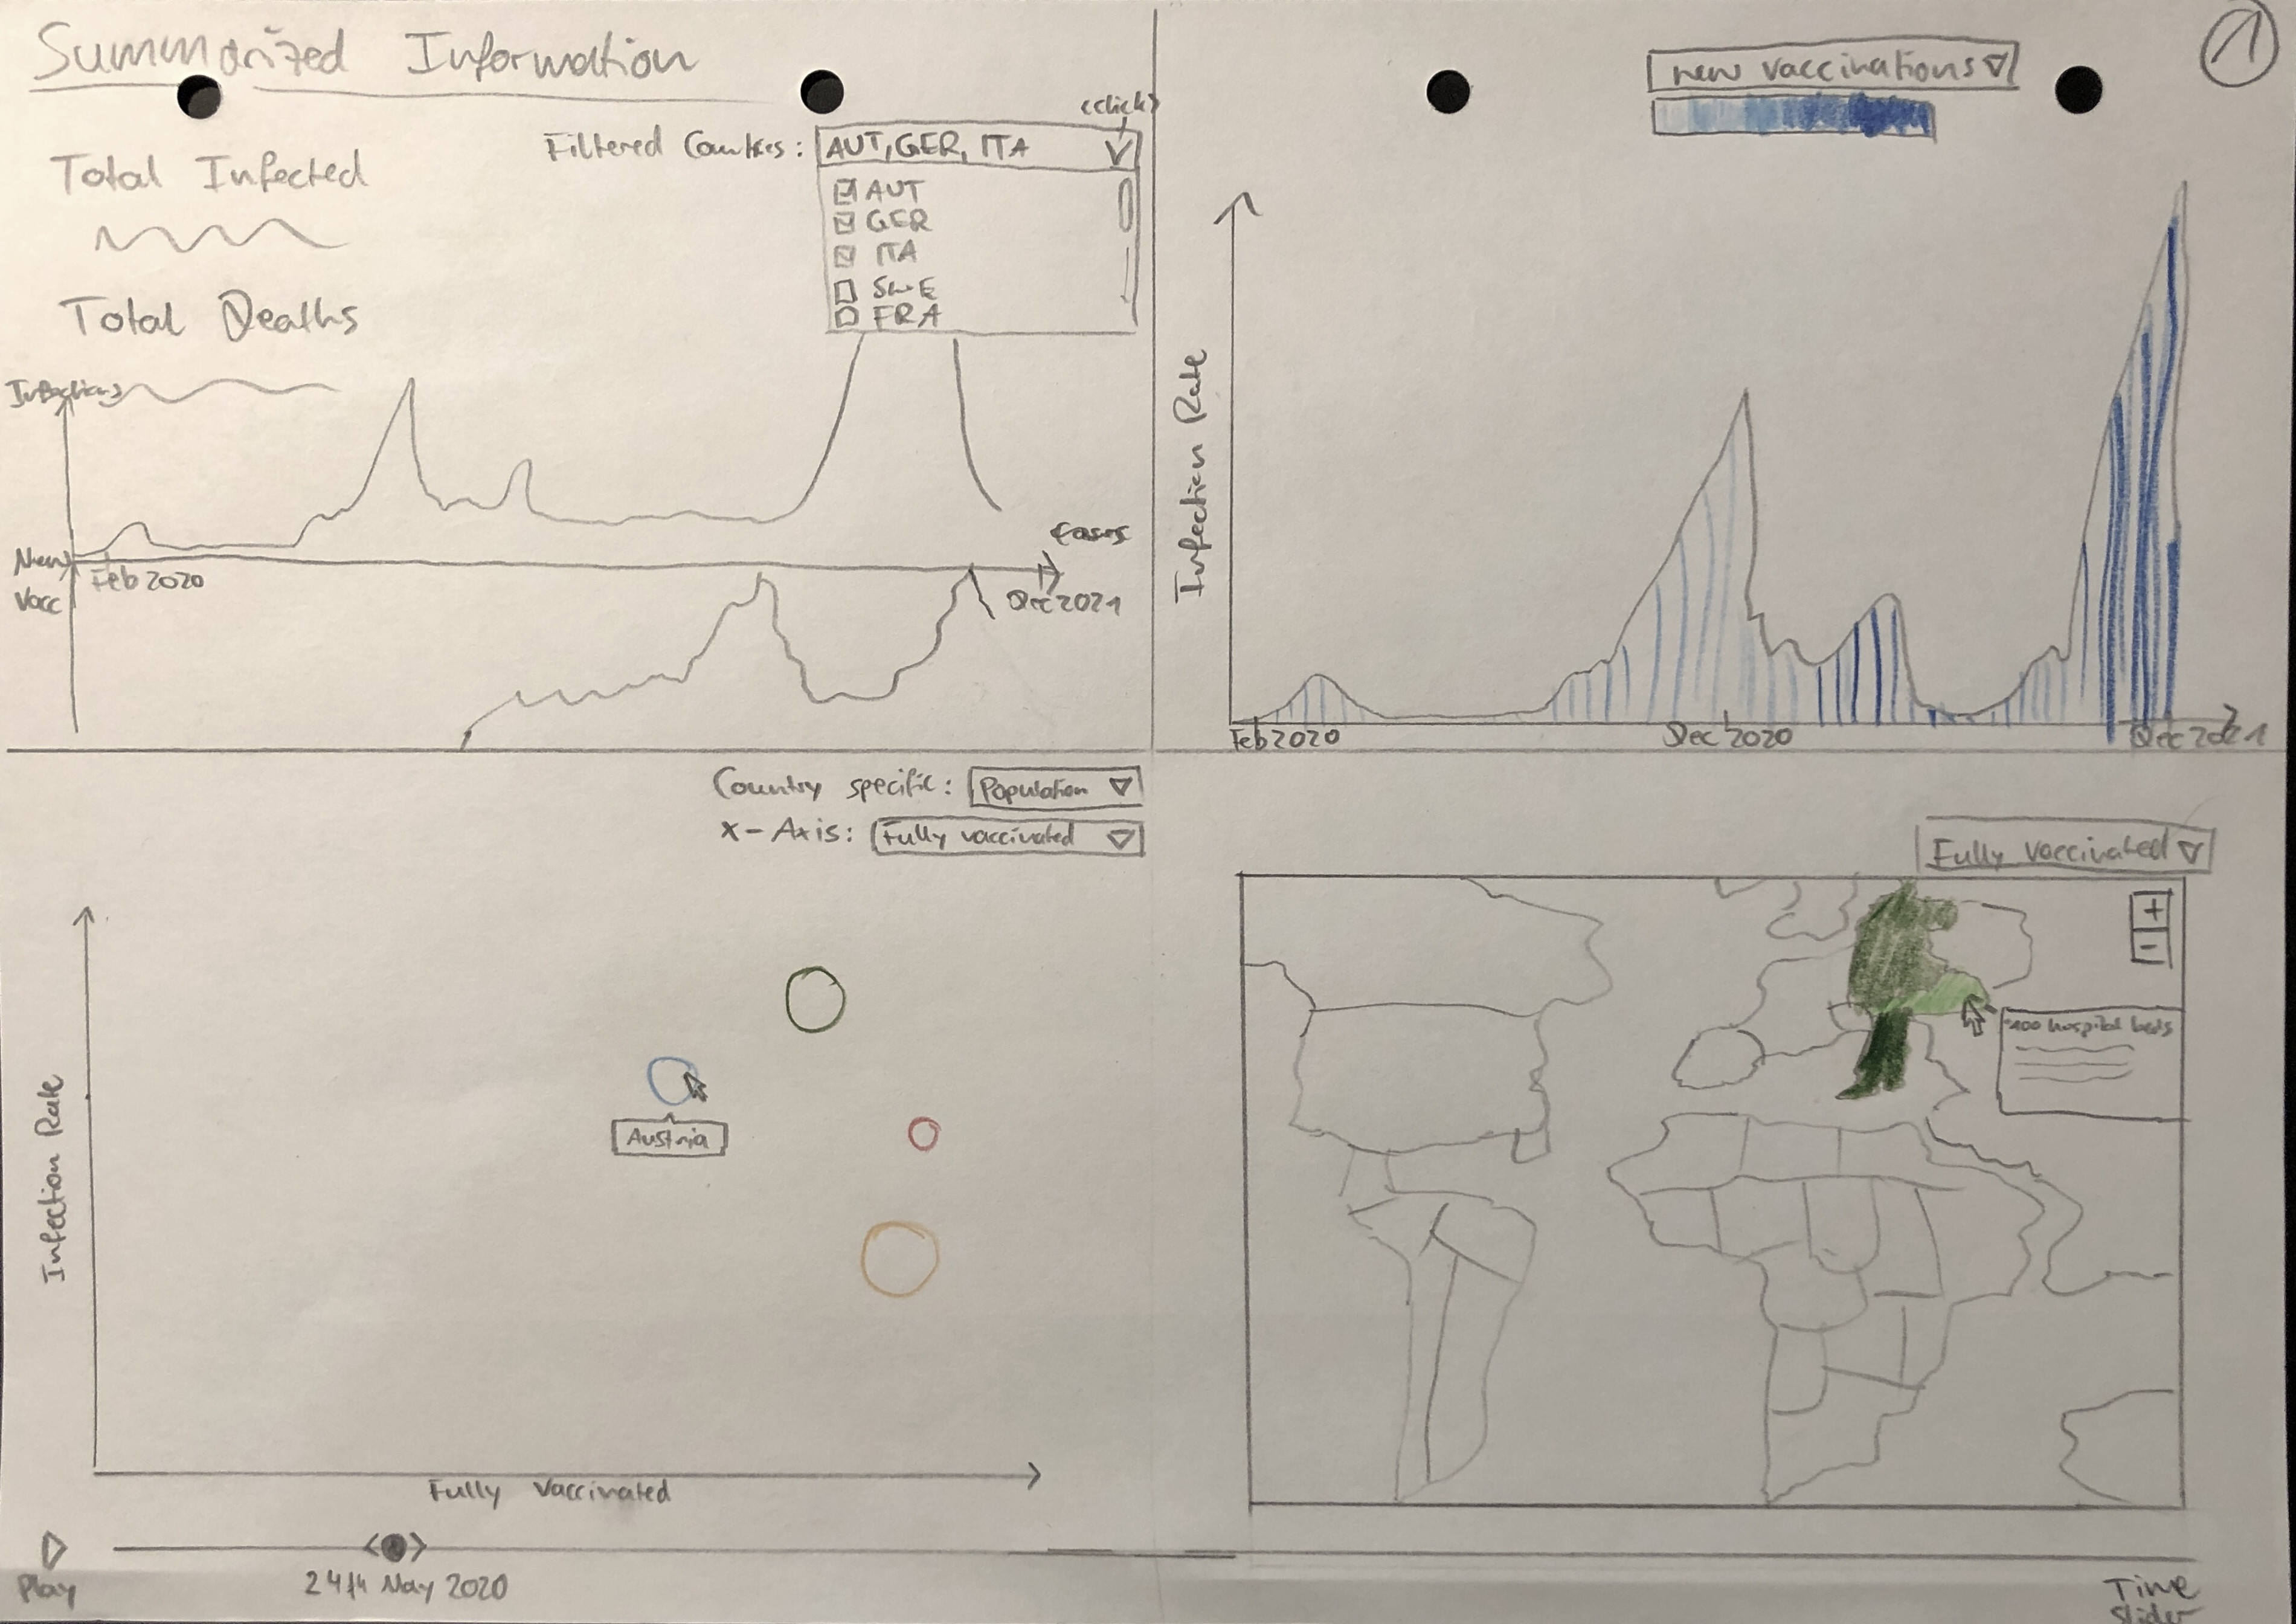
\includegraphics[width=\linewidth]{images/design10.jpg}
    \caption{Sketch for the first design variant.}
    \label{fig:design10}
\end{figure}

\subsection{Map centric dashboard}
\label{sec:design2}
Because a lot of tasks are based on comparing different values of different countries, my second design makes the map the center of the dashboard in order to 
either get an overview of a large area (Public Health) or focus on a single region (Government Official), which now works as the view which holds 
it all together (Section~\ref{sec:abstraction} (T4)) and is also responsible for selecting and highlighting countries as well as presenting the user a slider 
which changes the currently selected date on the map view and the view on the lower right. 
In addition to that, this view also offers the user another option of showing data on the map. A checkbox on the lower end of this view activates the encoding 
of another variable. After clicking and selecting a feature (e.g. the population density), each countries' coordinates change to a size representing the chosen 
feature (see also Figure~\ref{fig:design20} and~\ref{fig:design21}). 
By hovering a country, a tooltip shows additional information on that country.
\\\\
The view on the lower right as well as the bar chart diagram on the upper right are the same as in section~\ref{sec:design1}, because especially the lower view 
seemed like a perfect fit for satisfying the needs of both user's goals (Section~\ref{sec:abstraction} (T2) and (T3))
\\\\
The view on the left works like a preferences view, which -- besides showing cumulative data and corresponding graphics (Section~\ref{sec:abstraction} (T5)) --, 
is also responsible for filtering data, whiche again affects all other views as well (Section~\ref{sec:abstraction} (T1) and (T5)). In addition to that, 
statistical data like population density, median age, etc. are shown by clicking on country names. 

\begin{figure}[!htb]
    \centering
    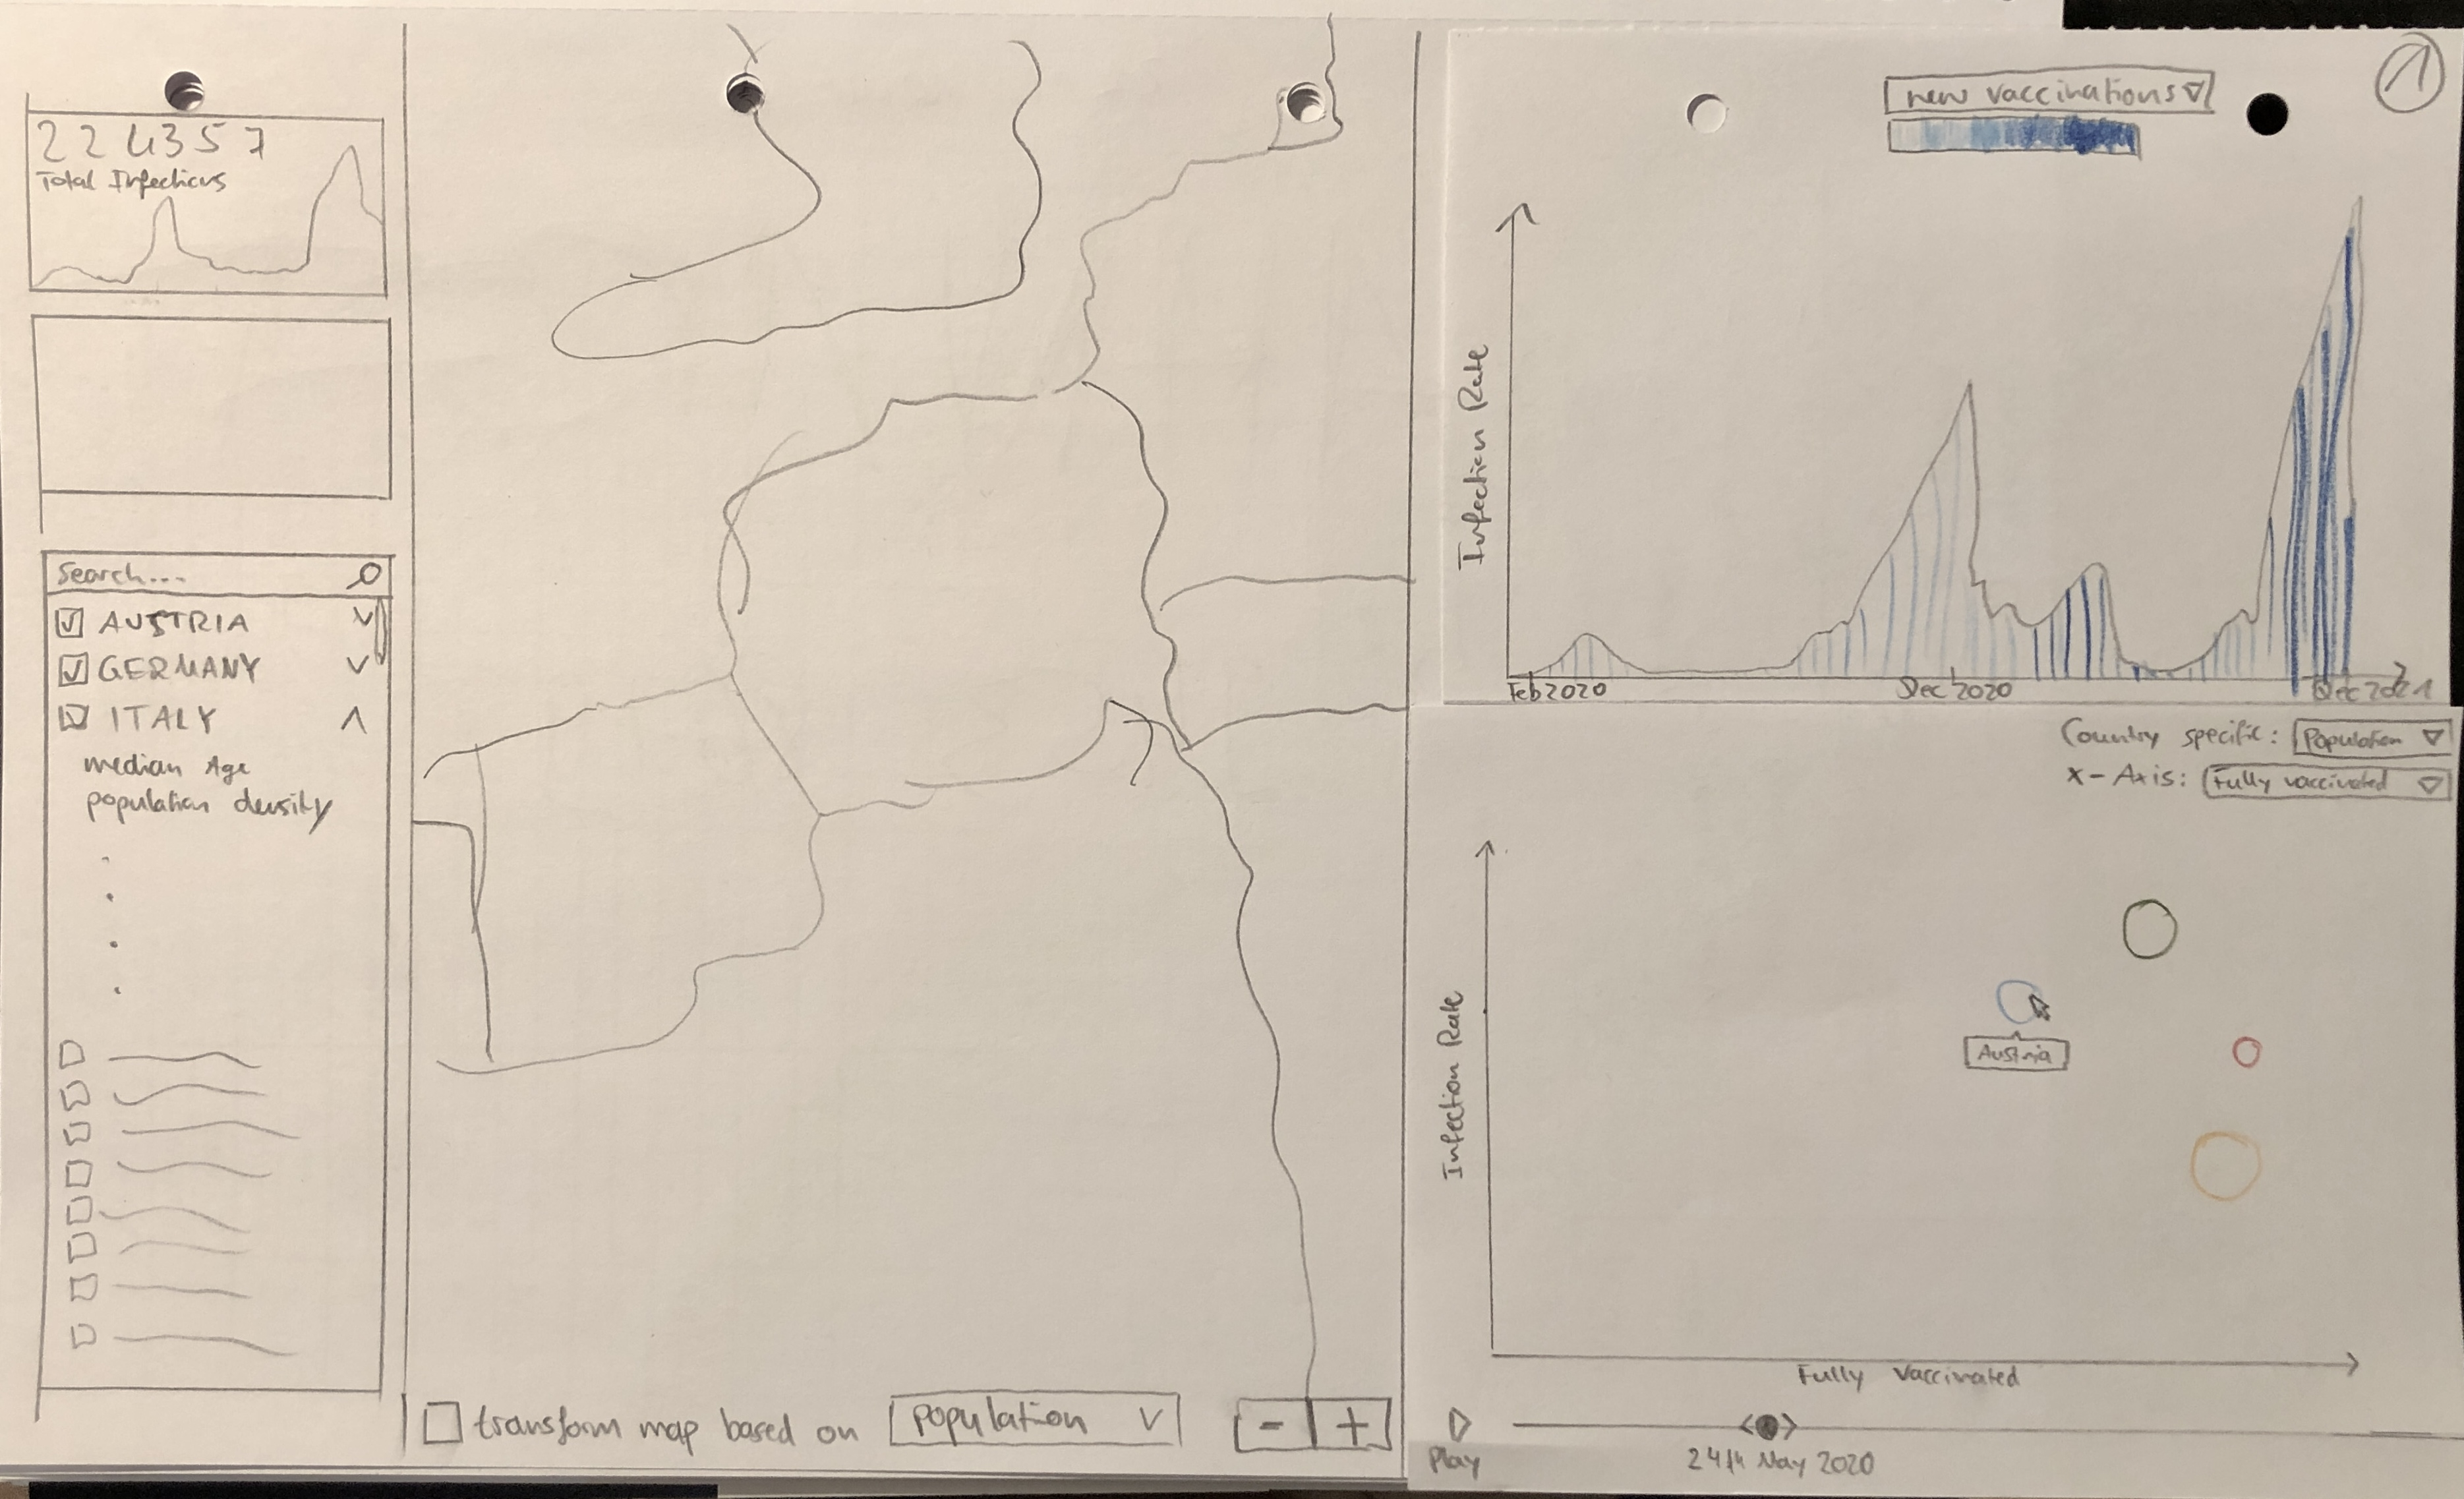
\includegraphics[width=\linewidth]{images/design20.jpg}
    \caption{Sketch for the second dashboard design.}
    \label{fig:design20}
\end{figure}

\begin{figure}[!htb]
    \centering
    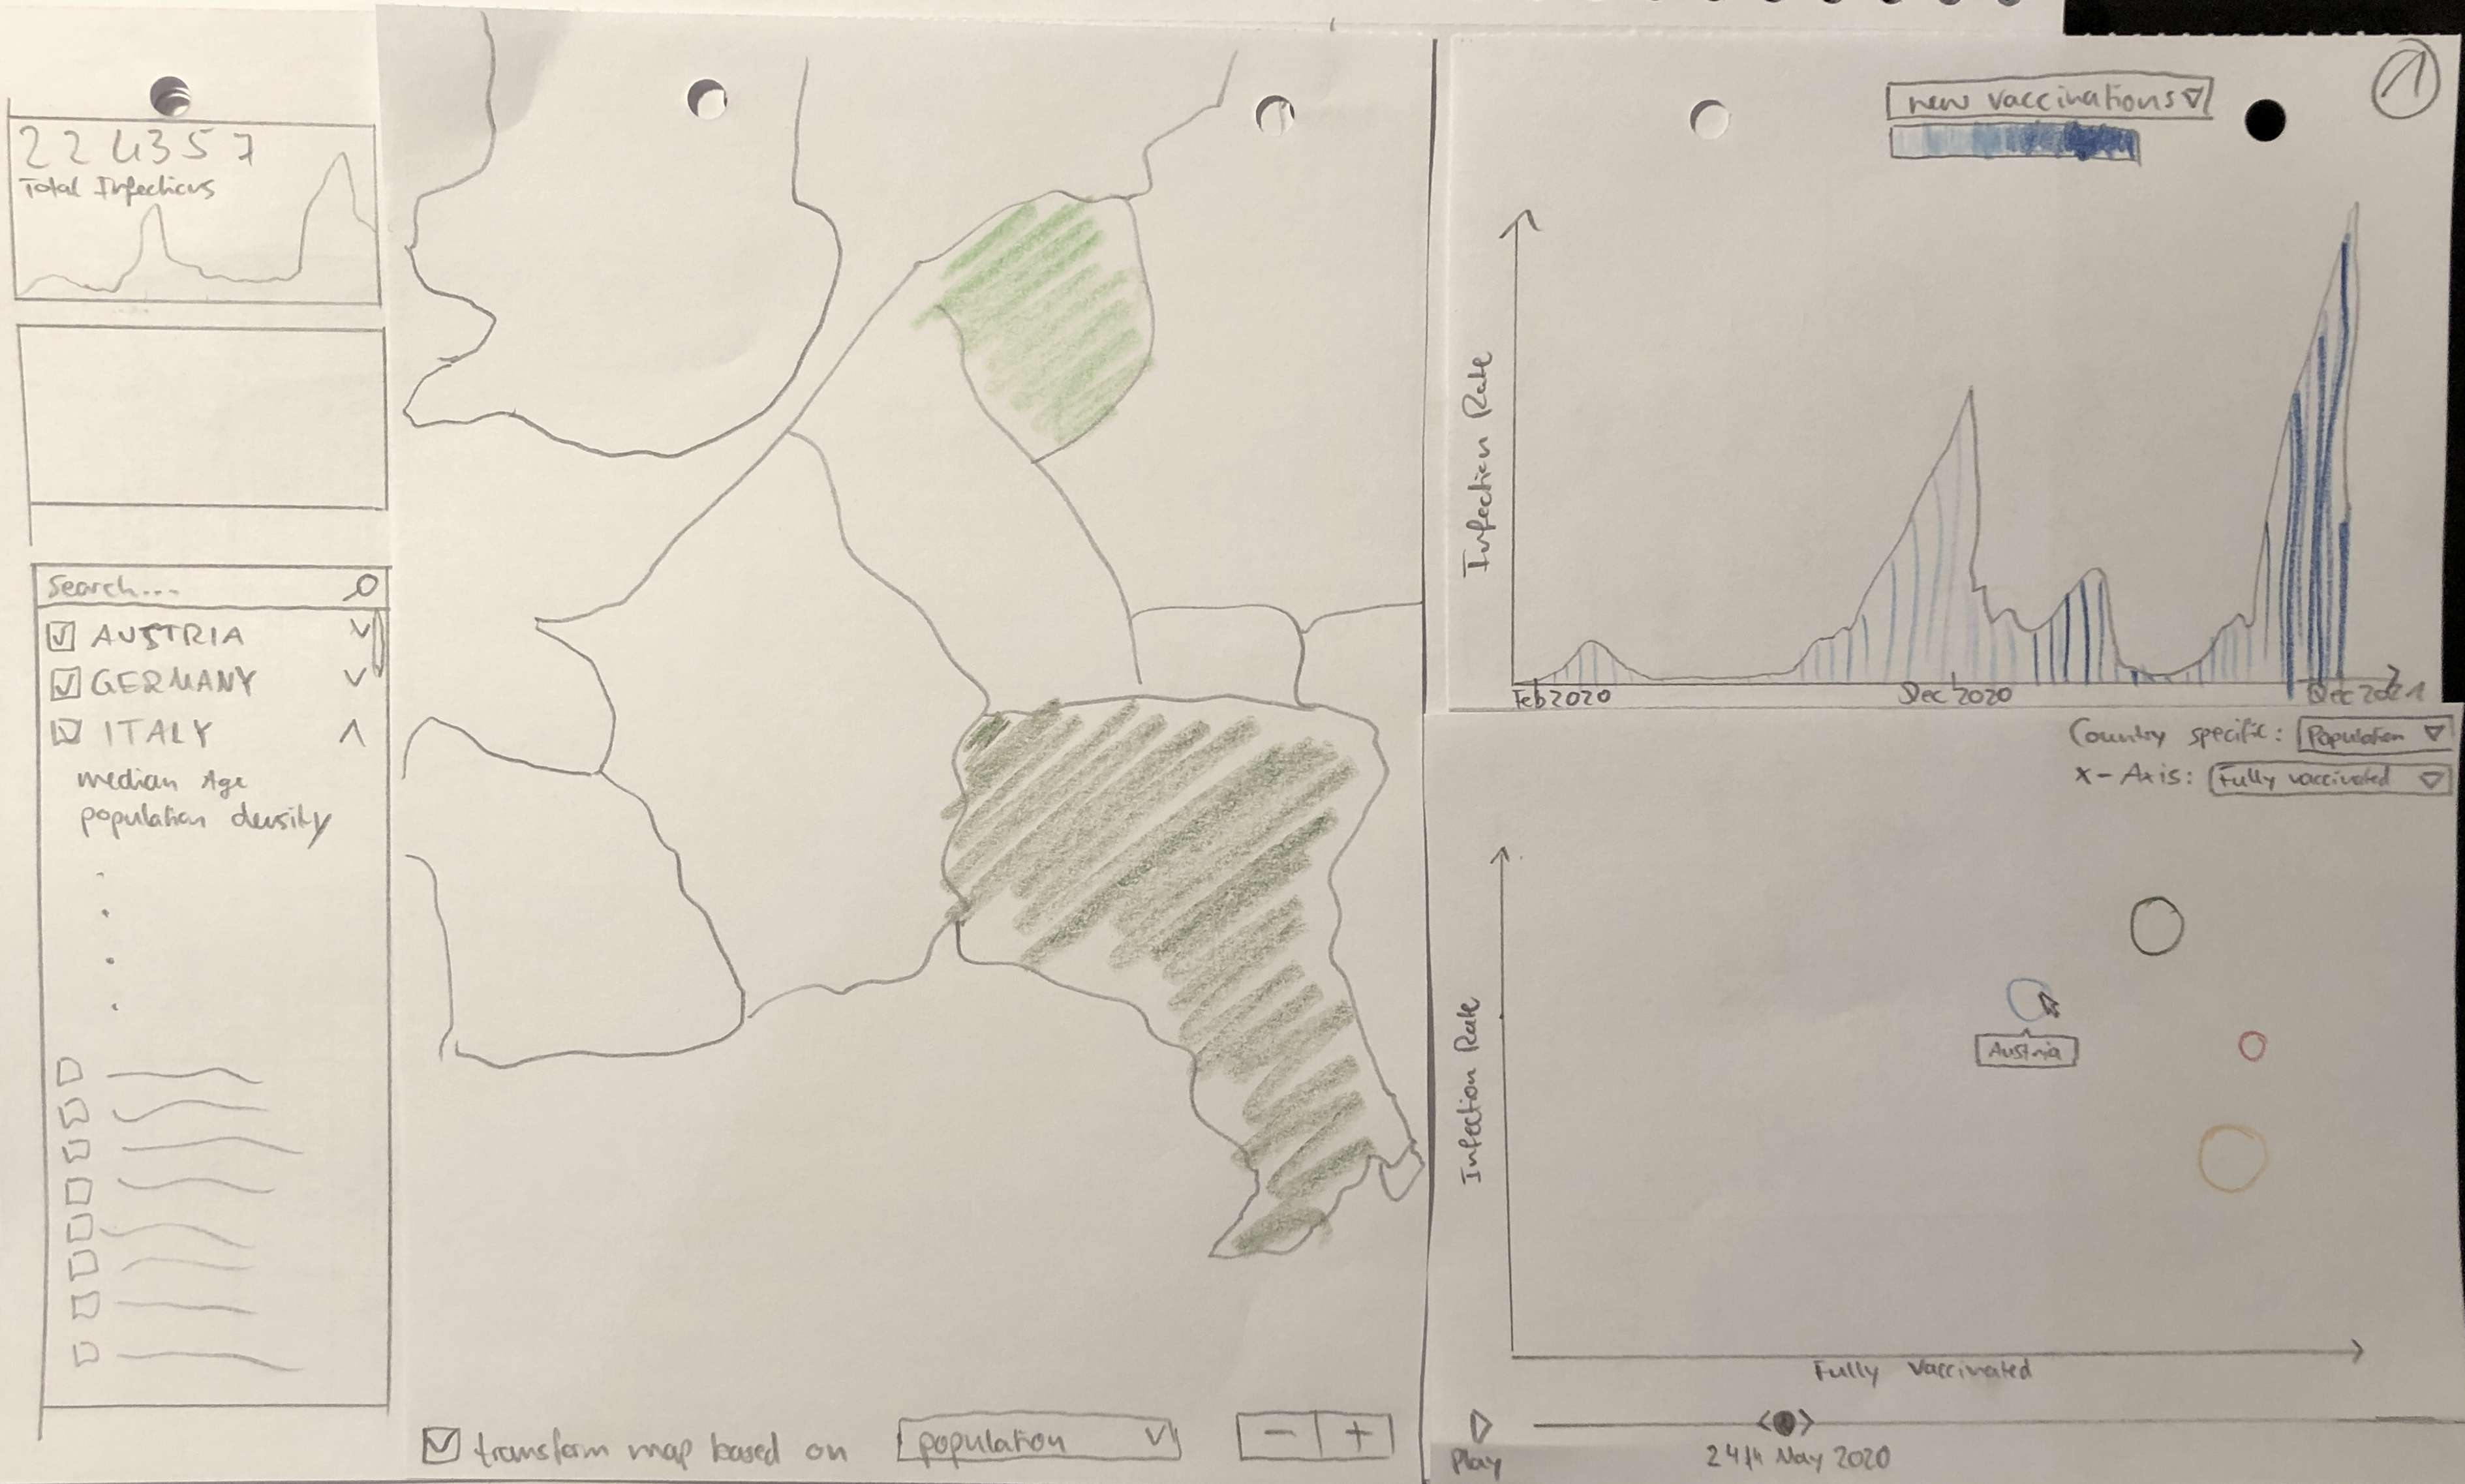
\includegraphics[width=\linewidth]{images/design21.jpg}
    \caption{Transformed world map based on selected variable "population density" in the second dashboard design. This option morphes the coordinates of 
    countries based on another variable.}
    \label{fig:design21}
\end{figure}

\section{Comparison}
When designing visualizations of complex or simply a lot of different features, there is always the risk of overloading graphics with too much information or giving 
too much freedom to the user in deciding which data features are shown on the visualization. This was particularily a difficult tradeoff when designing the 
lower left visualtion in section~\ref{sec:design1}, where five different variables are encoded in the visualization. The infection rate and a choosable feature are 
displayed on the x and y-axes, color encoding is used for distinguishing the countries, the size of the circles for another feature and in addition to that, the 
position and size can also be changed when using the time slider on the very bottom of the dashboard. I still decided to do it for the following reasons:

\begin{itemize}
  \item Two-dimensional graphics are relatively common and familiar to most eyes, which makes it easy to grasp connections between features.
  \item Mosf often, not all countries are selected, but rather only a small subset (aditionally limited by the dashboard itself.).
  \item Showing the change over time is not the main goal of this view.
\end{itemize}

If a user especially wants to see time-related data over the timespan of the whole pandemic, he will be able to use the bar chart for displaying multiple 
features as well.
The main advantage of the second design, however, is the map centric design. It works as an overview, so that the user always has the selected 
region on the map in sight but can focus on either specific information about a single country on the left or get a deep insight into correlating features 
on the right at the same time.
This is turn, is a major flaw of the first design (equally balanced views in terms of size), as users can be easily overwhelmed by the sheer amount of 
different information and data, whereas in the second design the map acts as an anchor for the whole dashboard. 
\\\\
Therefore, the second design of section~\ref{sec:design2} would be my final choice.


\section{Conclusion}
Again, the number of different features measuring the impact of the COVID-19 pandemic like the reproduction value, 7-day smoothed infections, used intensive 
care unit beds can be overwhelming and confusing. In order to solve this, my map-centric approach can help in making filtering easy by selecting countries visually, 
comparing fixed variables of countries visually by the morphed version of the map, getting specific information on a country by clicking it as well as 
discovering trends over time and correlation between several choosable features.
\\\\
In addition to that, all these benefits come with only four different main views, whereas other online available dashboards need a much larger number 
of visualizations to transfer the same amount of information to multiple user types.

\end{document}

